\chapter{Page layout and whitespace}\label{sec:layout}


%
%
%
\section{How \TeX{} sets lines}\label{sec:overfull}\label{sec:babel}

The line and paragraph shaping algorithm of \TeX{} has long been touted as excellent.
The algorithm breaks lines and hyphenates words in a way that tries to
keep the inter-word spacing visually pleasing.
It works on paragraph level: changing a word may cause the preceding lines to be set differently,
as \TeX{} tries to find the globally best solution.

\begin{technote}
The algorithm has quite a few parameters that \emph{can} be modified\dots{}
but most likely \emph{should} not.
You can find them in the \TeX book \cite{texbook}.
\end{technote}

\begin{warning}
The following discussion is \TeX nical, and mostly for giving you an idea of how things work.
If you find yourself needing to manipulate boxes directly,
\begin{enumerate}
    \item reconsider what you are doing,
    \item go read the \TeX book.
\end{enumerate}
\end{warning}


\TeX{} lays out a line just like a human typesetter would do with metal type.
The basic unit is \emph{box}, a rectangular piece of content.\index{boxes}
\TeX{} alternates between a horizontal mode, where the boxes are set in line,
and a vertical mode, where boxes are set on top of each other.%
\footnote{To be precise, there are two horizontal modes:
the one where lines are broken automatically, and the one where they are not.
Similarly, there are two vertical modes that differ in page breaking behaviour.
Finally, there are the inline and display math modes, bringing the total to six.}
Boxes are nested to produce complicated layouts.

\begin{technote}
We can play an old-school typesetter with the \obscmd{hbox} and \obscmd{vbox} commands.
(These are low-level \TeX{} commands -- see below for \LaTeX{} versions!)
%
\begin{VerbatimOut}{\jobname.tmp}
\vbox{\hbox{\hbox{Above1}\hbox{Above2}}\hbox{Below}}
\end{VerbatimOut}
\ShowExampleBelow
\end{technote}

A key concept in typesetting is the \emph{baseline}.\index{baseline}
The bottoms of letters lay on the baseline.
Some letters like `p' have \emph{descenders} that drop below the baseline.
The \emph{height} of a letter is the vertical extent above baseline;
the \emph{depth} that below baseline.
%
\begin{center}
\newcommand\ExampleText{\normalfont\fontsize{48pt}{48pt}\selectfont Typography}
\newlength\Myheight
\settoheight\Myheight{\ExampleText}
\newlength\Mydepth
\settodepth\Mydepth{\ExampleText}
%
\begin{tikzpicture}
    \small
    \draw (0cm,0) -- (9cm, 0) node[right] {baseline};
    \draw[dotted] (0cm,\Myheight) -- (9cm,\Myheight) node[right] {line height};
    \draw[dotted] (0cm,-\Mydepth) -- (9cm,-\Mydepth) node[right] {line depth};
    \draw (0,0) node[right,anchor=base west] {\ExampleText};
\end{tikzpicture}
\end{center}

The height of each line is given by the \emph{baseline skip}:
the vertical distance between baselines.
It is visually pleasing when lines are spread evenly,
but \TeX{} will happily give extra space when content like $\dfrac 1 2$ needs it,
even though it looks bad (just look at it!).
Moreover, the baseline skip might vary between pages,
since \TeX{} might try to squeeze one more line onto a page to get a better layout.

Back to boxes.
I can invent three reasons to create boxes manually:
\begin{itemize}
    \item overriding hyphenation,
    \item drawing a frame around something,
    \item doing some placement tricks.
\end{itemize}
We will look at each of these use cases.
You can create your own boxes with the \cmd{mbox} command,
and framed boxes with the \cmd{fbox} command.
These commands are both defined in \LaTeX{}.
%
\begin{VerbatimOut}{\jobname.tmp}
\fbox{Framed!}
\end{VerbatimOut}
\ShowExample
%
The \verb|\fboxsep| length parameter determines the padding between the box and the frame;
by default it is 3~pt.
There is also a \verb|\fboxrule| parameter for the width of the line (0.4~pt by default).
We can use these parameters to illustrate how \TeX{} lays out words (ignoring hyphenation):
%
\begin{VerbatimOut}{\jobname.tmp}
\setlength\fboxsep{0pt}

\fbox{Some} \fbox{example} \fbox{text}
\fbox{that} \fbox{forms} \fbox{a}
\fbox{complete} \fbox{example}
\fbox{paragraph}.
\end{VerbatimOut}
\ShowExample

The \cmd{makebox} and \cmd{framebox} commands behave otherwise similarly,
but they accept optional width and alignment parameters.
By default, the text is centered.
Inside these commands and their arguments,
a special \cmd{width} command gives the total width of the contents.

Do note that lines are not automatically broken inside these boxes.
You can thus overflow the size:
%
\begin{VerbatimOut}{\jobname.tmp}
\framebox[4cm][c]{Centered}\\
\framebox[1.5\width][r]{Some legroom}\\
\framebox[1cm][l]{Overflowed it!}
\end{VerbatimOut}
\ShowExample

\begin{technote}
There are a few \emph{niche} use cases for producing special layouts with boxes.
You most likely should not use these in an article.

The first is that you can take advantage of the overflow with zero-width boxes.
Here we use a right-aligned zero-width box to push stuff into the margin:
%
\begin{VerbatimOut}{\jobname.tmp}
Some text\\
\makebox[0pt][r]{(!) }Important text\\
Some more text
\end{VerbatimOut}
\ShowExample

Another is to raise or lower a box for dramatic effect:
%
\begin{VerbatimOut}{\jobname.tmp}
My feeling \raisebox{-\totalheight}{sank.}
\end{VerbatimOut}
\ShowExample
%
The \cmd{totalheight} command gives the height of the line:
it is the sum of \cmd{height} (of the contents above baseline)
and \cmd{depth} (of the contents below baseline).
We will talk about baseline a bit later below.
\end{technote}


What if you want to put multiple lines of content into a box,
with automatic hyphenation?
Enter paragraph boxes.\index{boxes!paragraph}
The \env{minipage} environment essentially creates a page within page.
You need to tell it the width of the box, and optionally whether the
top, center, or bottom line is aligned with the baseline:
%
\begin{VerbatimOut}{\jobname.tmp}
Some text
\begin{minipage}[b]{2.7cm}
interrupted by a rambling
note, followed by
\end{minipage}
some
\begin{minipage}[t]{2cm}
more text, albeit not
very usefully set either.
\end{minipage}
\end{VerbatimOut}
\ShowExampleBelow
%
Let us also show a more practical example of how this could be used:
%
\begin{VerbatimOut}{\jobname.tmp}
\begin{minipage}[c]{5cm}
\textbf{Curriculum Vit\ae}\\
Cira the dog\\
Born 2009\\
Expert eater of everything
\end{minipage}
\hfill
\begin{minipage}[c]{4cm}
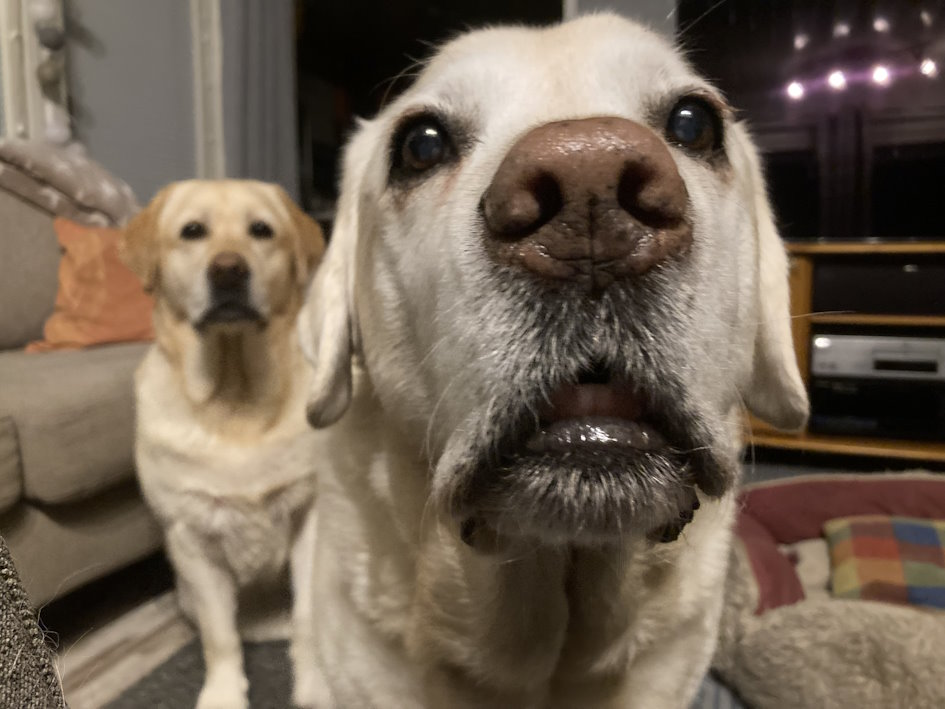
\includegraphics[bb=2.8cm 1.4cm 7cm 6cm, clip, width=\textwidth]
    {pictures/TheDogs.jpg}
\end{minipage}
\end{VerbatimOut}
\ShowExampleBelow


Finally, let us talk about invisible boxes.

The \cmd{phantom} command can be used to reserve space.
You can see it in action in \Cref{sec:math split}.
%
\begin{VerbatimOut}{\jobname.tmp}
There is a \phantom{phantom} in here.\\
There is a phantom in here.
\end{VerbatimOut}
\ShowExampleBelow

The \cmd{rule} command creates a filled box,
but it can also be used to create a \emph{strut}:\index{strut}
an invisible ``support beam'' that takes up some vertical space.
The command takes the width and height of the rule,
optionally preceded by the position above baseline:
%
\begin{VerbatimOut}{\jobname.tmp}
Thick rule on baseline: \rule{1cm}{3pt}\\
Raised a bit: \rule[6pt]{1cm}{3pt}
Below baseline: \rule[-3pt]{1cm}{3pt}
\end{VerbatimOut}
\ShowExample
%
If we set the width to zero, then the space is reserved but no rule is drawn.
Here we reserve 0.5~cm below the baseline and 1~cm above it:
%
\begin{VerbatimOut}{\jobname.tmp}
\fbox{\rule[-0.5cm]{0pt}{1.5cm}%
A lot of room!}
\end{VerbatimOut}
\ShowExample
%
This can be used e.g.\ to create some vertical clearance inside a table cell.



%
%
\subsection{Hyphenation}
By default \TeX{} hyphenates words according to a set of English rules.
It is very good at hyphenating general text, and can be trusted at it.%
\footnote{As a non-native English speaker, I don't even know what the rules are.}
Sometimes, especially with technical compound words, it might still need some help.

To hint the possible breaking points, use the \cmd{-} command.
This disables automatic hyphenation for the particular word,
so it will only be broken at the hinted points.
Conversely, if a word should not be broken across lines, it can be wrapped in an \cmd{mbox}.
Finally, to prevent a line break between two words,
the tilde \verb|~| symbol produces a \emph{non-breaking space}.

Compare these two passages (to illustrate the automatic hyphenation, they are slightly different).
The breaking override commands cause the lines to be underfull,
but at least for names the result is syntactically more correct.
%
\begin{VerbatimOut}{\jobname.tmp}
Quantum electro\-chromo\-dynamics
presented by P.~Laarne,
based on \mbox{Chatterjee}.\\

Quantum electrochromodynamics
presented by one P. Laarne,
reading about Chatterjee.
\end{VerbatimOut}
\ShowExample

\begin{practices}
If you add a hyphenation hint to a word,
I suggest adding \verb|\-| commands at all reasonable hyphenation points.
That might save you some effort when the line breaking changes.
\end{practices}

\todo{Adding words to the hyphenation dictionary}

Let us then talk about the issues.
An \emph{overfull hbox}\index{overfull} means that \TeX{} could not break the lines
without overflowing into the margin.
Conversely, an \emph{underfull hbox}\index{underfull} results from a line having too little content,
and thus unacceptably large spaces between words.
There are a few ways to fix these issues:

\begin{itemize}
    \item If the offending line is visually not too bad, just accept it.
    \item Slightly change the wording or word order to create better hyphenation opportunities.
    \item Manually tweak the hyphenation of a long word within the paragraph.
    \item If the page layout causes suboptimal paragraph shaping,
        it could also be tweaked, but this is an extreme action (see \Cref{sec:paragraph layout}).
\end{itemize}
%
There is just one hard rule:

\begin{warning}
Only fix over-/underfull issues at the very end of publication process,
when you have applied the final style file
and all the content fixes are done.

Since the \TeX{} layout algorithm is global,
adding just one letter can change the breaking of a line,
which can change the length of the paragraph,
which can change the page layout,
which then propagates to the next pages.
Result: You fixed a typo, and all the fine-tuning you had done on the following pages was just lost.

I have often seen a one-word change increase the length of a paper by half a page.
\todo{TLC production notes}
\end{warning}

By default \LaTeX{} produces justified text that extends from the left to right margin.
It is possible to let the line lengths vary (as most word processors do by default).
This is done by the \cmd{raggedright} command,
or more locally inside a \env{flushleft} environment.
%
\begin{VerbatimOut}{\jobname.tmp}
Here the text is spread evenly
between the two margins.
Spaces between words can vary a lot.\\

\raggedright

Now the lines are broken
once they no longer fit more text.
Spaces between words are more equal.
\end{VerbatimOut}
\ShowExample
%
Using ragged lines is a design decision,
and only applicable to documents where you are in control.
There seems to be quite a lot of disagreement of the merits of justified and ragged text.

I personally used ragged text in the bibliography of my MSc~thesis,
as the justification made it a mess of overfull and underfull lines.
Some journals have also made this choice.
Your mileage may vary.



%
%
\subsection{Language}

The standard method for producing \LaTeX{} documents in a language other than English,
or even in multiple languages, is the \pkg{babel} package.
It does several things:
\begin{itemize}
    \item Applies the language-specific hyphenation rules;
    \item Translates words produced by \LaTeX{} commands such as ``Chapter'', ``References'',
        and dates produced by \cmd{today};
    \item Might do some typographical fine-tuning.
\end{itemize}

The list of languages is passed as an option when \pkg{babel} is loaded.
The last language on the list is taken to be the default language for the document.
In these notes, the magic command is
%
\begin{ExampleCode}
\usepackage[finnish,french,english]{babel}
\end{ExampleCode}
%
The full list of languages (and regional variants!) can be found in the babel documentation.
Some European languages have undergone major orthography revisions in the past decades;
for modern German the language code is \verb|ngerman|
and for Norwegian nynorsk it is \verb|norsk|.

The currently active language is changed with \cmd{selectlanguage}.
The \env{otherlanguage} environment can be used for a short passage in a different language.
Below there are two visible changes:
obviously the language is different, but do note also the small space before !\ in the French version.
\indexcmd{frquote}
\begin{VerbatimOut}{\jobname.tmp}
This file was compiled on \today.
``Awesome!''\\

\begin{otherlanguage}{french}
Cet fiscier est compilé le \today.
\frquote{Voilà!}
\end{otherlanguage}
\end{VerbatimOut}
\ShowExample

The hyphenation rules are also changed,
but the effect might be negligibly small.
Overall, the hyphenation algorithm of \TeX{} is optimized for English,
so the long Finnish words might need your help.
\begin{VerbatimOut}{\jobname.tmp}
Pitkähköjen yhdyssanamuotojen tavutus
oikeinkirjoitussääntöjen mukaisesti\\

\begin{otherlanguage}{finnish}
Pitkähköjen yhdyssanamuotojen tavutus
oikeinkirjoitussääntöjen mukaisesti
\end{otherlanguage}
\end{VerbatimOut}
\ShowExample

Finally, since non-English languages also contain non-English characters,
we need to talk about font encodings.

\begin{gotcha}\label{rem:font encoding}
This here is the most important place where the traditional pdfTeX compiler
and the Unicode-native LuaTeX and XeTeX compilers differ.
You \emph{should always} use the \cmd{fontencoding} command with pdfTeX,
unless your document only contains the basic English characters.
On the other hand, you \emph{should not} use \cmd{fontencoding} with LuaLaTeX or XeLaTeX,
since they use a better internal encoding by default.

It is not dangerous to use \cmd{fontencoding} with the new compilers,
but you might get suboptimal \todo{clarify} behaviour.
\end{gotcha}

Since 2018, \LaTeX{} has accepted Unicode input by default.
However, this only applies to the input:
characters are then transformed into an internal representation
and further into individual glyphs from a font file.%
\footnote{To be precise, several characters can be combined into one glyph:
see the ffi in `efficient'.
These are called ligatures.}
When \TeX{} and \LaTeX{} were developed,
they had to solve the problem of having many (mathematical) glyphs,
but Unicode was back then far from a universal standard.

There are several of these internal representations,
and the so-called \verb|OT1| encoding is the most recent one.

The LuaTeX and XeTeX engines use Unicode for their internal representation,
so this command is no longer necessary.
Furthermore, it conflicts with \todo{what exactly},
so it should be removed altogether.

\begin{practices}
Unfortunately, most journals (and coauthors)
still use pdfLaTeX in their production process,
so you might just need to accept the minor issues with newer compilers.
\end{practices}



%
%
%
\section{Units of measure and whitespace}

\TeX{} supports specifying distances in a variety of units.
The most useful are:
\begin{description}
    \item[\texttt{cm}] Centimetres
    \item[\texttt{in}] Inches (1~in=2.54~cm)
    \item[\texttt{pt}] Points (1~in=72.27~pt); usually used for font sizes%
        \footnote{There is also the \texttt{bp} (big point) used by PDF format,
        where there are exactly 72~bp to an inch.}
    \item[\texttt{ex}] Approximate height of `x' in current font
    \item[\texttt{em}] Approximate width of `M' in current font
    \item[\texttt{mu}] Math unit (1~em=18~mu); used for spacing in math mode
\end{description}
%
Wherever a length is used, it must be supplied with a unit: for example, \verb|1.5cm|.

In horizontal mode, a space is created with the \cmd{hspace} command.
The \cmd{quad} command produces an \emph{em space} (1~em), \cmd{qquad} doubly so,
and \cmd{enspace} half of it.
In math mode, there are some more commands: see \Cref{sec:math spacing}.
%
\begin{VerbatimOut}{\jobname.tmp}
An em space is this big:\\
xxx\hspace{1em}xxx
\end{VerbatimOut}
\ShowExample


It is possible to make a length \emph{stretchy},\index{strectch}
letting it expand or shrink within some limits.
Here the syntax \texttt{1cm plus 1cm minus 0.6cm} means that
the space can be anything between 0.4~cm and 2.0~cm:
%
\begin{VerbatimOut}{\jobname.tmp}
\newcommand\spa
  {\hspace{1cm plus 1cm minus 0.6cm}}

Every\spa word\spa space\spa in\spa this\spa
long\spa example\spa paragraph\spa has\spa
this\spa weird\spa stretchy\spa space.
Perhaps\spa anybody\spa should\spa not\spa
set\spa any\spa text\spa like\spa it.
\end{VerbatimOut}
\ShowExample

An extreme case of stretchy spaces is given by \cmd{hfill}:
it expands to take all the available space on the line.
%
\begin{VerbatimOut}{\jobname.tmp}
Left\hfill center\hfill right
\end{VerbatimOut}
\ShowExampleBelow
%
Internally, \cmd{hfill} is implemented as \verb|\hspace{\stretch{1}}|.
With the \cmd{stretch} command it is possible to distribute the space in uneven ratio:
%
\begin{VerbatimOut}{\jobname.tmp}
Left\hspace{\stretch{1}} off-center\hspace{\stretch{2}} right
\end{VerbatimOut}
\ShowExampleBelow

There are also the \cmd{hrulefill} and \cmd{dotfill} commands
that fill the space with something:
%
\begin{VerbatimOut}{\jobname.tmp}
Left\hrulefill center\dotfill right
\end{VerbatimOut}
\ShowExampleBelow

The same general ideas work for vertical spacing.
One can request exact vertical space with \cmd{vspace} or a stretch space with \cmd{vfill}
(below, the latter does nothing since the ``page'' streches according to the example content):
%
\begin{VerbatimOut}{\jobname.tmp}
Something

\vspace{1cm}

Something else

\vfill

Bottom of the page
\end{VerbatimOut}
\ShowExample

Instead of manual spacing commands,
you should use the semantically more meaningful
\cmd{smallskip}, \cmd{medskip}, and \cmd{bigskip} commands.

However, there is a significant catch.
Remember that \TeX{} alternates between the horizontal and vertical mode.
Using vertical commands in the horizontal mode might cause some surprises.
%
\begin{VerbatimOut}{\jobname.tmp}
An example.
\bigskip
Inside this paragraph,
there is a vertical spacing command.
Can you see where it got applied?
\end{VerbatimOut}
\ShowExample


%
%
\subsection{Length variables}

Like counters, \TeX{} supports special length variables.
\TeX{} and \LaTeX{} supply quite a lot of read-only variables that can be used in length expressions.

Let us use \cmd{textwidth} as our example.
It gives the width of the text area on the page.
We can print its value with the \cmd{the} command (mostly useful for debugging!),
and put a multiplicative factor in front of it:
%
\begin{VerbatimOut}{\jobname.tmp}
The text width is \the\textwidth.
Here's a line of that width:

{\color{blue}\rule{\textwidth}{1pt}}

And of half that width: {\color{blue}\rule{0.5\textwidth}{1pt}}
\end{VerbatimOut}
\ShowExampleBelow

Importantly, this length changes depending on the context.
Inside a \env{minipage} environment, the width of the text area is different.
Let us do the same example again, but now the output is placed inside a smaller minipage:
%
\begin{VerbatimOut}{\jobname.tmp}
The text width is \the\textwidth.
Here's a line of that width:

{\color{blue}\rule{\textwidth}{1pt}}

And of half that width:
{\color{blue}\rule{0.5\textwidth}{1pt}}
\end{VerbatimOut}
\ShowExample

Out of the box, the only calculation possible with lengths is multiplication,
like \verb|0.5\textwidth| used above.
The \pkg{calc} package has traditionally been used when a complete expression language is needed.

\begin{latexthree}
\LaTeX3 now also provides similar functionality through the \cmd{dimeval} and \cmd{inteval} commands:
%
\begin{VerbatimOut}{\jobname.tmp}
Text height: \the\textheight\\
Paper height: \the\paperheight\\
Padding:
\dimeval{\paperheight - \textheight}\\
About this many lines:
\inteval{\textheight / \baselineskip}
\end{VerbatimOut}
\ShowExample
%
Be warned that the syntax does have some peculiar corner cases.
\end{latexthree}


It is usually enough to provide length expressions to commands,
but sometimes it is useful to define custom length variables.
Such a variable is initialized with \cmd{newlength}, similar to how counters are created.
It can then be set with \cmd{setlength}, and used by prefixing the name with \verb|\|:
%
\begin{VerbatimOut}{\jobname.tmp}
\newlength\Mylen
\setlength\Mylen{1.75em}

My\hspace{\Mylen}space.
\end{VerbatimOut}
\ShowExample

\begin{technote}
Like counters, length variables live in the global scope.
Once created, they never go away.
\end{technote}

There are the useful \cmd{settowidth}, \cmd{settoheight}, and \cmd{settodepth}
commands that measure a piece of text and store its size in the variable:
%
\begin{VerbatimOut}{\jobname.tmp}
\settowidth\Mylen{Hello world!}

The text ``Hello world!''
is {\the\Mylen} wide.

\settowidth\Mylen{\large Hello world!}

In \verb|\large| font it takes
the whopping \the\Mylen.
\end{VerbatimOut}
\ShowExample



%
%
%
\section{Page geometry}

Let us then move on to the layout of a complete page.
To see the frame of a page, you can load the \pkg{showframe} package
or pass the \verb|showframe| option to the \pkg{geometry} package.
The result is shown in \Cref{fig:page geometry}.

\begin{figure}
\centering
\setlength\fboxsep{0pt}
\fbox{\includegraphics[totalheight=0.8\textheight]{examples/geometry.pdf}}
\caption{The geometry of an A4~page. The header is set to be 15~pt tall.}
\label{fig:page geometry}
\end{figure}

The most basic customization tools are the options passed to the document class.
For further changes to the geometry, or a larger range of paper sizes,
it is easiest to turn to the \pkg{geometry} package.

Just loading the \pkg{geometry} package changes the layout:
by default, the package applies narrower margins than \LaTeX{} does by default.
Further customization is done by optional arguments to the package,
or later in the preamble with the \cmd{geometry} command.

You only need to specify the options you specifically want to customize
-- the package computes the remaining parameters.%
\footnote{Of course, it is possible to give an incompatible set of measurements.}
For all the details, look at the package documentation.
Some of the more useful options are:
\begin{description}
\item[\texttt{inner}] The width of the inner margin.
    In \verb|oneside| document mode, this corresponds to the left margin.
\item[\texttt{outer}] The width of the outer margin.
    In \verb|oneside| document mode, this corresponds to the right margin.
\item[\texttt{textwidth}] The width of the text area.
\item[\texttt{textheight}] The height of the text area.
\item[\texttt{lines}] Alternatively to the above,
    the desired text height in lines (in the current default font).
\item[\texttt{headheight}] The height of the header area.
\item[\texttt{headsep}] Distance between the header and text area.
\item[\texttt{footskip}] Distance between the text area and the footer.
\item[\texttt{paper}] This accepts an extended range of paper sizes:
    \verb|a0paper| through \verb|a6paper|, and the same for B and C series.
    Custom sizes can be specified through \verb|paperwidth| and \verb|paperheight|.
\end{description}

\begin{remark}
University of Helsinki doctoral theses are printed on B5~paper.
The suggested font size is 10~pt in that case.
\end{remark}

\begin{warning}
The raw \TeX{} and \LaTeX{} lengths are available as well,
and many a Stack Exchange answer suggests modifying them directly.
There is nothing wrong with it, but \pkg{geometry} gives a nicer interface
that avoids some surprising things.
\end{warning}

\begin{technote}
As an example of a surprise, the coordinate system of \TeX{}
puts the origin at 1~inch to the right and below of the top-left corner of the paper.
That means that some of the internal length parameters are negative.
\end{technote}


Of the read-only length variables provided by \LaTeX{},
\cmd{textwidth} and \cmd{textheight} are some of the most useful ones.
It is very common to set a figure to be a certain portion of the text width.


%
%
\subsection{Landscape pages}\label{sec:landscape pages}

\LaTeX{} has several restrictions to changing the layout mid-document.
Some parameters can be customized with the \cmd{newgeometry} command,
which ends the current page, outputs all the outstanding floats,
and starts a new page with the new layout.

Sometimes, it is useful to produce single landscape pages, e.g.\ to hold a wide table.
For this, you can use the \pkg{pdflscape} package
and its \env{landscape} environment.
The contents of this environment are set on a new landscape page (or several).
See also \Cref{sec:landscape floats} for automatic placement of floats on landscape pages.

\begin{technote}
The \textsf{pdf} in \pkg{pdflscape} stands for the fact
that the environment even tells the PDF reader application to rotate the page on your screen.
This is its sole improvement over the older \textsf{lscape} package.
\end{technote}



%
%
\subsection{Paragraphs and page breaks}\label{sec:paragraph layout}

Other two commonly customized parameters are \cmd{parindent} and \cmd{parskip}.
As the names suggest, they control the indentation and distance between paragraphs.

By default, paragraphs are indented, with no extra vertical separation.
If you prefer non-indented, vertically separated paragraphs, the commands are:
%
\begin{VerbatimOut}{\jobname.tmp}
\setlength\parindent{0pt}
\setlength\parskip{4pt}

Some text forming an example paragraph.
Just enough to get it to a few lines.

Another example paragraph,
with quite a few words.
\end{VerbatimOut}
\ShowExample

If you want to remove the indentation of a single paragraph only,
you can put \cmd{noindent} at the beginning of the paragraph.

\bigskip

Let us then move to page breaks.
The \cmd{clearpage} command ends the current page,
then produces enough pages to set all the outstanding floats (figures and tables),
and finally starts a new page.
The \cmd{cleardoublepage} variant ensures that the new page has odd number,
which puts it on the right-hand side of a twoside layout.
This is done automatically at the end of chapter in the \textsf{report} document class.

Generally, you should not otherwise interfere with the page breaking algorithm,
but sometimes it is necessary for a good layout.
The \cmd{pagebreak} command forces a manual page break.

However, this command \emph{is dangerous}.
If the preceding text changes, it is possible that the \cmd{pagebreak} command now produces
a mostly-empty page!

Instead, it might be better to use the \pkg{needspace} package.
The identically named command approximates the remaining space on the page,
and starts a new page if there is not enough.
For example, to ensure that there is space for two more lines,
one can say
%
\begin{ExampleCode}
\needspace{2\baselineskip}
\end{ExampleCode}

Finally, there is an extreme command for fine-tuning the final layout of a page.
The \pkg{addlines} package can be used to add or remove lines to the current spread.
(The package applies the extension to both sides of a spread in twoside mode;
in oneside mode it only affects the single page.
This distinguishes the package from raw \LaTeX{} \cmd{enlargethispage} command.)

\begin{warning}
Only do fine-tuning to the page layout at the very end of editing process
-- even the tiniest change can cause a massive cascade of layout changes!

Quite often, you can do completely without these tweaks.
\end{warning}


%
%
%
\section{Headers and footers}

\todo{Page numbering, lastpage}

\todo{General headers and footers}

\begin{remark}
The package gives a warning if the header height is not large enough.
The warning even gives a suggested value for the \cmd{headheight} length,
which you can pass to \pkg{geometry} (or do a raw \verb|\setlength|, if not using the package).
\end{remark}
